\documentclass[12pt]{article}

\usepackage[T1]{fontenc}
\usepackage[utf8]{inputenc}
\usepackage[estonian]{babel}
\usepackage[a4paper]{geometry}
\usepackage{hyperref}
\usepackage{url}
\usepackage{multirow}
\usepackage{float}
\usepackage{graphicx}
\usepackage{todonotes}
\usepackage{graphicx}
\usepackage{listings}
\usepackage{bm}
\usepackage{amsmath}

\restylefloat{table}


\usepackage{chapterbib}

\lstset{
    language=XML,
    morekeywords={encoding, bookstore, book, title, author, year, price, category}
}

\usepackage[
    round,
    authoryear,
    sort&compress,
    sectionbib
]{natbib}
\newcommand{\bi}[1]{\bf{\emph{{#1}}}}
\renewcommand{\refname}{Kasutatud kirjandus}
\AtBeginDocument{\renewcommand{\harvardand}{\&}}
\setcitestyle{aysep={,}}

\usepackage{titlesec}
\titlelabel{\thetitle\ }
\renewcommand\thesection{\arabic{section}.}
\renewcommand\thesubsection{\thesection\arabic{subsection}.}

\usepackage{enumitem}
\setlist[itemize]{topsep=-1pt}
\setlist[enumerate]{topsep=-1pt}
\setlist[description]{
   leftmargin=14pt,
   labelindent=14pt,
   topsep=-1pt
}

\setlength{\parindent}{0pt}
\setlength{\parskip}{10pt}

\def\autor{Kristiina Vaik}
\def\pealkiri{Eesti morfoloogiliselt märgendatud lapsekeele korpus}

\graphicspath{{figures/}}

\begin{document}

\begin{titlepage}
    \begin{center}
        {\large TARTU ÜLIKOOL}\\[0.3cm]
        {\large HUMANTITAARTEADUSTE JA KUNSTIDE VALDKOND}\\[0.3cm]
        {\large EESTI JA ÜLDKEELETEADUSE INSTITUUT}\\[0.3cm]

        \vfill
        {\large \autor}\\[0.3cm]
        {\large \textbf{\pealkiri}}\\[0.3cm]
        {\large Magistritöö}

        \vfill
        \begin{center}
        {\large
            Juhendajad: Heiki-Jaan Kaalep ja \\
            Virve-Anneli Vihman
        }
        \end{center}
        \vfill
        {\large TARTU \the\year}
    \end{center}
\end{titlepage}

\tableofcontents

\newpage
\cleardoublepage
\phantomsection
\addcontentsline{toc}{section}{Sissejuhatus}
\section*{Sissejuhatus}


SEE KOKKUVÕTE OLI SEMINARITÖÖ JAOKS. SEEGA, SEE POLE SEE ``PÄRIS'' KOKKUVÕTE. JA PEALKIRJAD ON KA ALLES ÜSNA ALGELISED.\\

Seminaritöö eesmärgiks on teha lühike sissejuhatus magistritöö vaid ühe praktilise väljundi kohta, milleks on eesti morfoloogiliselt märgendatud lapsekeele korpus. Korpuse tekstid pärinevad CHILDES-i eesti lapsekeele alamkorpustest. Morfoloogiliselt märgendatud lapsekeele korpuse loomine oleks väga vajalik, sest CHILDES-i tööriistad ei võimalda teha eesti keele jaoks automaatset morfoloogilist analüüsi.
 
Töö koosneb kahest peatükist. Esimeses peatükis räägitakse lähemalt korpusest, selle liigitusvõimalustest ja arengutendentsidest. Lisaks antakse lühiülevaade sellest, mida korpuse märgendamisel silmas tuleb pidada, ja millised korpused juba Tartu Ülikoolis olemas on. Teises peatükis kirjutatakse morfoloogiliselt märgendatud lapsekeele korpuse loomise probleemidest. Tutvustatakse CHILDES-i korpust ja kuidas on seal esindatud eesti keele alamkorpused. Lõpuks tehakse väike ülevaade alamkorpuste standardiseerimise probleemidest.

\newpage
\section{Lapsekeel ja sellele iseloomulikud jooned}
Siin: Reili Argus ja võimalusel ka muudki.


\subsection{MINGI PEALKIRI}

Eesti keele morfoloogia on rikkalik, kuid selle omandamine on keerukas protsess. Keele omandamisel tuleb lisaks reeglipärastele mallidele omandada ka ebareeglipärased mallid ning teada, kuidas toimuvad tüvesisesed muutused (astme- ja lõpuvaheldus) ning milliseid morfoloogilisi formatiive (tunnused ja lõpud) tuleb tüve külge lisada. 
Konstruktivistlik lähenemine jagab morfoloogiasüsteemi omandamise kolme perioodi (Dressler 2003: 9-10) VIIDE:

\begin{itemize}
    \item Premorfoloogiline omandamine- etapp, millal lapse keeles esinevad morfoloogilised muuted, kuid morfoloogiline süsteem pole lahus kognitiivsetest struktuuridest;
    \item Protomorfoloogiline periood- etapp, mil hakkab arenema morfoloogiline produktiivsus. Laps loob omale grammatika, mis on täiskasvanutest reeglipärasem ja pisem, kuid siiski abistab omandamist siis, kui muutemorfoloogia süsteem pole veel selge. Toimub esimeste reeglite ja analoogiaseoste loomine. Alguses keskendutakse erinevatele vormidele, mis muutuvad teatud kategooriate prototüüpideks;
    \item Täiskasvanute morfoloogia omandamine- etapp, mil keelesüsteemi allmoodulid hakkavad omavahel koostööd tegema. Sel ajal hakkavad lapsel aktiivselt välja kujunema muutmissüsteemid, sealhulgas liitmine ja tuletamine.
\end{itemize}

Esimesed poolteist eluaastat tegelevad lapsed sisendkeele dešifreerimisega ehk püütakse öeldule tähendust omistada. Morfeemide hulk keeles on väga suur, seega pole 
laps võimeline korraga kõiki morfeeme ära õppima ning selle tõttu keskendutakse pigem sagedasematele ja esilduvamatele morfeemidele. Olulised tegurid morfeemide valiku juures on sagedus, segmenteeritavus, morfeemi asend tüves ning selle allomorfide esinemise seaduspärasused. (Argus 2004: 16, Argus 2008: 19) VIIDE Esmalt peab laps selgeks saama kust algab ja lõpeb sõna. Esmalt omandatakse lühikesi lahtiseid silpe, kuna neid on lihtsam hääldada ja segmenteerida kui kinniseid. Kõnejada segmenteerimist ja silbipiiri ära tundmist hõlbustab reduplikatsioon, mis on hoidjakeelele väga omane (ta-da, ai-ai jne). Hoidjakeele rutiinsed väljendid aitavad lapsel aru saada, kust algab samasugune foneetiline realisatsioon. Reduplikatsioon aitab mõista sõnu kui mitmest osast koosnevast tervikust, mis omakorda aitab hilisemas etapis tajuda sõnavormis esinevat muutumatut (tüvi) ja muutuvat (tunnused ja lõpud) osa. Reduplikatiivsed sõnad hõlbustavad morfoloogia omandamist, sest tunnuseta vorme hakatakse tasapisi asendama morfoloogilisi elemente sisaldavate üksustega. Reduplikatsioon aitab omandada ka eesti keelele iseloomulikku kõnetakti ehk trohheust, mille puhul ühest lahtisest silbist tekitatakse kahesilbiline keeleüksus, kus vahelduvad rõhuline ja rõhuta silp. Enne kahe aastaseks saamist on lapse kõnes enamik keeleüksuseid trohheilise rütmiga. (Argus 2008a: 19-20) VIIDE

Premorfoloogilisel etapil omandavad lapsed vorme terviklike üksustena, ilma et toimuks tüve ja tunnuse analüüsimist. Sel perioodil esineb laste kõnes kõige rohkem tunnusteta kahesilbilisi sõnu. Pikemates vormides, kas loobutakse rõhutust ehk viimasest silbist (nt \emph{sitikas} > \emph{siti}, \emph{traktor} > \emph{takku}/\emph{takka}), \emph{rebane} > \emph{repa} või jäetakse käändelõpp ära ja kasutatakse selle asemel genitiivi tüve (nt \emph{poti} > \emph{potile}). Kahesilbiliste vormide kasutust võib vaadata nii eelistuse kui ka piiranguna. Piirang selles mõttes, et laps ei pruugi olla suuteline hääldama pikemates sõnades teatud rõhutut silpi. Eelistus selles mõttes, et laps eelistab kahesilbilisi sõnu, kuna need on sisendkeeles kõige sagedasemad. Nii eesti kui ka soome keeles on lapsekeele uurijad märganud, et on perioode, mil laps pikendab ühesilbilise sõna kahesilbiliseks, nt \emph{lutt} > \emph{luti}, \emph{pai} > \emph{paia}. Näiteid on ka sellest, et liitsõnade omandamisel püütakse eelistada kahesilbilisi sõnu, nt \emph{jõuluvana} > \emph{jõvvu}. Vahetult enne protomorfoloogilist etappi lõpeb kahesilbiliste sõnade periood. (Argus 2008a: 20–21) VIIDE

Kinniste silpide omandamine toimub nende hääldamise raskuse tõttu hiljem. Eesti keeles toimub kinniste esimeste silpide omandamine kinnistest järgsilpidest varem. Leidub näiteid, kus kinnise järgsilbiga sõnu mugandatakse trohheiliseks, nt \emph{viiul} > \emph{villu}/\emph{illu}, \emph{ämber} > \emph{ämpu}, \emph{põrr} > \emph{põrra}. Premorfoloogilisele etapile on iseloomulik, et lapse kõnes kinnise järgsilbi lõppkonsonant on ära jäetud, kuna laps ei kasuta selliseid käände- ja pöördelõppe, mis muudaksid järgsilbi kinniseks. Näiteks, partitiivi lõpp -\emph{t} jääb hääldamata (\emph{küpsist} > \emph{kispi}), mitmuse nominatiivi lõpp -\emph{d} jääb hääldamata (\emph{mammud} > \emph{mammu}), inessiivi lõpp -\emph{s} jääb hääldamata (\emph{vannis} > \emph{vanni}, \emph{aias} > \emph{aia}). Konsonandi hääldamine sõltub paljuski konsonandi positsioonist: sõnaalguline konsonant jääb tavaliselt alles, kuid sõnalõpuline konsonant mitte. Kinnise järgsilbi hilisem omandamine on ootuspärane, kuna eesti keeles on kahesilbilised lahtised lõppsilbiga sõnad väga sagedased. (Argus 2008a: 22) VIIDE


Reili Argus (2008a: 23)VIIDE kirjutab, et võiks justkui eeldada, et morfoloogilised formatiivid ja õiges astmes välte valimine raskendab morfoloogilise süsteemi omandamist, aga selgub, et eesti keeles omandatakse produktiivsed vältevaheldusmallid (nõrgeneva tüvega ühesilbilised substantiivid) juba premorfoloogilisel perioodil, mil ei ole tunnused ega lõpud veel omandatatud. Vältevaheldus omandatakse varakult, kuna vältevahelduslikud sõnad on sisendkeeles sagedased ning väldete opositsioonidel on grammatiliste tähenduste eristamisel tähtis roll. Näiteks nõrga- või tugevaastmelised sõnad eristavad lapse jaoks grammatilisi tähendusi- valdaja ja objekt või objekt ja asukoht. (Argus 2008a: 23) VIIDE

Lõpuvaheldusega seotud vigu esineb üleminekul premorfoloogiliselt perioodilt protomorfoloogilisele perioodile. Enim valmistab probleeme II-välteliste konsonantlõpuliste sõnade vormimoodustus. Peamiselt just selliste fonoloogiliselt keeruliste sõnadega (\emph{el}-, \emph{er}-lõpulised), kus laps väldib kolmest konsonandist koosnevat kaashäälikuühendit (nt *\emph{numbert}, *\emph{numberit} ’\emph{numbrit}’; *\emph{kahvelga}, *\emph{kahveliga} ’\emph{kahvliga}’). Raskusi on ka \emph{s}-lõpuliste sõnade vormimoodustusega (nt *\emph{kärbese} ’\emph{kärbse}’; *\emph{võõraseid} ’\emph{võõraid}’). Vigu esineb ka \emph{ne}-liiteliste sõnade vormimoodustusega, näiteks nominatiivkujulise tüve \emph{rebane} asemel kasutatakse *\emph{reba} ja genitiivivormina *\emph{rebali}. Olgugi, et Arguse poolt vaatluse all olevad lapsed olid vältevahelduse varakult omandanud, siis laadivaheldus koos lõpuvaheldusega nagu \emph{V} > \emph{me} põhjustas mõningaid raskusi. Näiteks oli laps ära õppinud vormi \emph{juhtmed} ning järgmiste vormide käänamine toimubki selle ühe vormi analoogial (ehk *\emph{juhtme} ’\emph{juhe}’; *\emph{juhtmet} ’\emph{juhet}’) ning hilisemas materjalis on näha, et lapse keelekasutusse tekib vorm *\emph{juhte} ’\emph{juhtme}’. See näitab, et laps on tajunud, et \emph{m}-häälik kaob, kuid ei oska seda veel õigesti kasutada. (Argus 2008a: 23–24) VIIDE

Lõpuvaheldus pole nii süsteemne kui astmevaheldus ja selle omandamine on raske, kuna tüvevahelduslike vormide puhul tuleb lõpufoneemide järjestust vahetada. Lihtsaim viis sõnade moodustamiseks on lõpuhäälikute lisamine, kuid vahel üldistatakse muutesufiksit ka sõnadele, kus see ei ole normikohane, nt \emph{kauss}: *\emph{kausi}-\emph{t} (partitiivi läbipaistva lõpu -\emph{t} üldistamine), \emph{tühi}: *\emph{tühja}-\emph{sse} (illatiivi läbipaistva lõpu -\emph{sse} üldistamine). Eesti keeles on noomenitel lõpuvaheldusmalle rohkem kui pöördsõnadel, mistõttu ei valmista pöördsõnade lõpuvaheldusmallid lastele ka probleeme. Näiteks sellised tüvevaheldused nagu \emph{sööme}: \emph{süüa}, \emph{lööb}: \emph{lüüa}, \emph{ei pea}: \emph{pidime} on omandatud veatult. (Argus 2008a: 24, 26-27, 2008b: 20) VIIDE

Reduplikatiivsuse kõrval on morfoloogia süsteemi omandamisel tähtis roll ka deminutiivtuletustel, mille käigus nihutatakse astmevaheldusega sõnad astmevahelduseta muuttüüpi. Näiteks \emph{kiisu} ja \emph{kutsu} saavad selle nihke tõttu partitiivi läbipaistva lõpu -\emph{t}: \emph{kiisu}-\emph{t}, \emph{kutsu}-\emph{t}. Siinkohal on hõlbustav tegur ka vormihomonüümia, sest tuletatud sõnad nihkuvad sellisesse muuttüüpi, kus nominatiivi- ja genitiivivormid on homonüümsed. Väidetakse, et samakujulised vormid soodustavad muuteparadigmade omandamist, kuid see võib olla ka pidurdavaks teguriks. Nimelt võib laps hakata käänama ka \emph{pesa}-tüüpi sõnu astmevahelduseta muuttüübi järgi, nt *\emph{muna}-\emph{t}, *\emph{saba}-\emph{t}.(Argus 2008a: 25, 2008b: 19-20) VIIDE

Lähemalt võiks natuke rääkida ka muutemorfoloogia arengust sõnaliigiti. Argus kirjutab (2008a), et morfoloogiasüsteemi omandamine toimub sõnaliigiti erineva kiirusega ja et mõnes keeles omandatakse noomeni morfoloogia kiiremini kui verbi morfoloogia. Seda on põhjendatud sellega, et noomenite puhul tuleb omandada vähem morfoloogilisi kategooriaid. Lisaks arvatakse, et verbe omandatakse teisiti, sest noomenite referentsiaalsust on kergem hoomata. Verbid on semantiliselt keerukamad ja on rohkem seotud keele süntaktilise struktuuriga. (Argus 2008a: 37)VIIDE Kasutuspõhise lähenemise järgi konstrueerivad lapsed grammatika sellest, mida nad kuulevad. Näiteks kui keeles on ülekaalus substantiivid, siis ainult sellepärast, et substantiivide esinemissagedus on sisendkeeles suur. 


<<<<<<< Updated upstream

 Melissa Bowerman annab oma loengusarjas ``Ten lectures on language, cognition and language acquisition'' (2010 VIIDE) ülevaate sellest, kuidas lapsed õpivad kaardistama keelelisi vorme (sõnad, morfeemid, sõnajärg konstruktsioonid jpm) ja nende tähendusi. Sellele küsimusele läheneti keeltevahelise võrdluse perspektiivist. Välja tuli see, et mõned keeled on verbi-``sõbralikumad'' kui teised. Näiteks inglise hoidjakeeles domineerivad noomenid, kuid on keeli, kus noomenite ja verbide kasutus on ühtlasemalt jaotunud, nt korea ja mandariini keel ning tseltali ja tsotsili keel. Nendes keeltes on objekti informatsioon peidetud verbidesse. Näiteks tseltali ja tsotsili keeles on mitu verbi söömise tähistamiseks ja vastava verbi valik sõltub sellest, mida süüakse. Seega verbid kannavad endas objekti kohta palju informatsiooni ja seetõttu muutuvad noomenid diskursuses vähem oluliseks. See, millise sõnaliigi muutemorfoloogia omandamine kiiremini toimub, oleneb sisendkeele eripärast ja on vägagi keelespetsiifiline. (Bowerman) VIIDE.
=======
JAMA:
Melissa Bowerman annab oma loengusarjas ``Ten lectures on language, cognition and language acquisition'' (2010 VIIDE) ülevaate sellest, kuidas lapsed õpivad kaardistama keelelisi vorme (sõnad, morfeemid, sõnajärg konstruktsioonid jpm) ja nende tähendusi. Sellele küsimusele läheneti keeltevahelise võrdluse perspektiivist. Välja tuli see, et mõned keeled on verbi-``sõbralikumad'' kui teised. Näiteks inglise hoidjakeeles domineerivad noomenid, kuid on keeli, kus noomenite ja verbide kasutus on ühtlasemalt jaotunud, nt korea ja mandariini keel ning tseltali ja tsotsili keel. Nendes keeltes on objekti informatsioon peidetud verbidesse. Näiteks tseltali ja tsotsili keeles on mitu verbi söömise tähistamiseks ja vastava verbi valik sõltub sellest, mida süüakse. Seega verbid kannavad endas objekti kohta palju informatsiooni ja seetõttu muutuvad noomenid diskursuses vähem oluliseks. See, millise sõnaliigi muutemorfoloogia omandamine kiiremini toimub, oleneb sisendkeele eripärast ja on vägagi keelespetsiifiline. (Bowerman) VIIDE.
>>>>>>> Stashed changes

Argus ja Kõrgesaar uurisid sõnaliikide jaotumist ja esinemissagedust lapse ja täiskasvanu vahelistes spontaansetes igapäevavestlustes. Sõnaliikide jaotusena kasutati traditsioonilist liigitust, onomatopoeetilisi sõnu ning ebaselgeid sõnu ja üneeme arvestati eraldi. 




KIRJUTA:
Sõnaliikide jaotumisest

?

Hodjakeele erijooned

Hodjakeel ja lapsekeel kui sotsiolektid




\newpage
\section{Suuline keel ja sellele iseloomulikud jooned}
Peamiselt Tiit Hennostelt.

\newpage
\section{Korpused}
Selles peatükis tehakse lühike kokkuvõte korpustest. Selgitatakse lähemalt mida mõeldakse korpuse ja muude
oluliste mõistete all. Kirjeldatakse lühidalt ajaloolist tausta. Peatüki teine osa annab ülevaate eesti keele korpustest. Viimasena keskendutakse korpuse märgendamisele ja sellega seonduvatele olulistele mõistetele.

\subsection{Mis on korpus?}
Enne arvutite kasutuselevõttu mõeldi keeleteaduses keelekorpuse all kui keelekogumikku, mida sai
keeleuurija (vastandina enda intuitsioonile) kasutada uurimustöö algmaterjalina. Tänapäeval mõistetakse
keelekorpuse all elektroonilisel kujul olevat tekstikogu, kuhu lisatakse tekste eesmärgiga, et need annaksid
tõepärase pildi keelest ja iseloomustaksid keele hetkeseisu või muutumist. Tekste valitakse korpusesse teatud kriteeriumite alusel ja need esinevad standardses elektroonilises formaadis. \citep[9]{KR}

Korpuste põlvkonnad:
\begin{enumerate}
\item põlvkond (ca 1960ndate lõpp--1980ndate lõpp): suletud, representatiivne, väike, valdavalt 80ndatel
tehtud, palju käsitööd panustatud. Nt Brown, LOB, Frown, kirjaliku eesti keele 80ndate aastate korpus;
\item põlvkond (valdavalt 1990ndate teises pooles ja 2000ndatel): avatud, suured tekstihulgad,
elektrooniliste publikatsioonide teisendamine ühtsele korpuse kujule. Nt eesti keele koondkorpus;
\item põlvkond: väga suur, automaatselt veebist korjatud ja ühtsele korpuse kujule teisendatud, nt etTenTen.
\citep{KT}
\end{enumerate}

Esimesed elektroonilised tekstikorpused olid Browni ja Lancaster-Oslo/Bergeni (LOB) korpused. Nendesse korpusestesse lisatud tekstid olid väga läbimõeldud ja koosnesid vaid ühest miljonist sõnast, mis pole tänapäeva korpuste mahtudega võrreldav. Põhjuseks oli muidugi tehnikaareng. Browni ja LOB-i korpuste loomise ajal polnud arvutite jõudlus ja mälu nii suur, et suudaks talletada ja töödelda rohkemat kui üht miljonit sõna.
Tänapäeval pole see enam probleemiks. Ligi 20 aastat olid nende korpuste koostamise põhimõtted olnud standardiks ka paljude teiste keelte korpuste loomisel, sealhulgas ka tänapäeva eesti kirjakeele baaskorpuse jaoks. Tänu tehnika arengule tekkisid võimalused
suuremate tekstikorpuste loomiseks. Näiteks, 1991. aastal tehti Inglismaal algust kahe suure projektiga: \emph{British National Corpus} (BNC) ja \emph{Bank of English} (BoE). BNC on suletud korpus, mille maht on 100 miljonit sõna. BoE on avatud monitorkorpus. BoE on mõeldud eeskätt leksikograafidele kasutamiseks.
 \citep[9--11]{KR}


\subsection{Eesti keele korpused}

Tänapäeva kirjakeele korpus sai alguse 80ndate aastate \emph{baaskorpusest}, mille standardiks on Browni ja LOB-i korpused. Eesti kirjakeele korpus on suletud ja representatiivne. Korpus koosneb ühest miljonist sõnast, tekstid pärinevad aastatest 1984--1987 ja on jaotatud kümnesse tekstiklassi. Baaskorpusega liituvad ka \emph{niitkorpused} ehk \emph{läbilõikekorpused} (1890--1990), mis on suletud ja osaliselt representatiivsed, kuigi neis on vähem tekstiklasse. Baas- ja läbilõikekorpustes on kokku umbes 4 miljonit sõna. (\citealp[14--15]{KR})

\emph{Koondkorpus} (sai alguse 1990ndatel) on teise põlvkonna avatud korpus, mis koosneb umbes 250 miljonist sõnast. Tekstiklassid ei ole kindlaks määratud. Korpus sisaldab palju ajalehetekste ja kasutatakse terviktekste (mitte katkendeid). Koondkorpuse alamhulk on \emph{Tasakaalus korpus}, mis sisaldab 5 miljonit sõna nii ilukirjandust, ajakirjandustekste ja teadustekste. Kolmanda põlvkonna korpused on automaatselt veebist korjatud, sisaldades foorumite, blogide ja kommentaariumide tekste. \citep[38]{M_OK2015} Eesti keele kolmanda põlvkonna korpuseks on \emph{eTenTen}, mis koosneb on 270 miljonist sõnast 686000 veebilehelt. \citep{eTenTen}

\emph{Paralleelkorpus} on korpus, mis sisaldab sama teksti vähemalt
kahes keeles, mille üksused on paralleelistatud. \emph{Paralleelistamine} tähendab paralleelteksti üksteise tõlkeks olevate osade märgendamist ehk pannakse paika, et millised laused, osalaused, fraasid on omavahel vastavuses. Tuntuim paralleelkorpus maailmas on Kanada \emph{Hansard}, mis koosneb inglise- ja prantsusekeelsetest parlamendidebattidest. Tartu Ülikoolis on tehtud eesti-inglise paralleelkorpus. Eesti keelt sisaldavaid paralleelkorpuseid on vähe. Eesti keelt sisaldab Soome paralleelkorpus \emph{SCLOMB}, mis sisaldab Läänemere-äärsete keelte tekste ja nende tõlkeid teistesse Läänemere-äärsetesse keeltesse. Keeletehnoloogia seisukohalt on paralleelkorpus väga oluline keeleressurss, nt saab paralleelkorpusi kasutada masintõlkesüsteemide loomisel ja sõnastike automaatsel genereerimisel.
(\citealp[17--18]{KR})


KAS MA PEAKS NEIST KORPUSTEST PIKEMALT KIRJUTAMA??\\
Eesti keele erikorpused:
\begin{enumerate}
    \item suulise kõne korpus;
    \item spontaanse kõne foneetiline korpus
    \item dialoogikorpus;
    \item murrete korpus;
    \item vana kirjakeele korpus;
    \item foneetikakorpus jne.\citep{Keelekogu}
\end{enumerate}


\subsection{Korpuse märgendamine}

SELLES ALAPEATÜKIS MA KAHTLEN, SEST SEE ON JUSTKUI LIIGA COPY-PASTE. JA MUL POLE TEGELIKULT JU TARVIS SÜNTAKTILISEST JA SEMANTILISEST TASANDIST RÄÄKIDA, FOOKUS ON SIISKI MORFOLOOGILISEL ANALÜÜSIL. PIGEM TEEKS ALAPEATÜKI MORFANALÜSAATORIST JA SELLE TEHNILISEST KÜLJEST.

Korpustest on kasu siis, kui vajalik info on sealt lihtsasti kättesaadav. Selleks, et korpus ei jääks lihtsalt elektrooniliste tekstide arhiiviks, oleks tarvis korpusesse esmalt interpretatiivset infot lisada. Seda protsessi nimetatakse \emph{korpuse märgendamiseks}. Korpuse märgendamise etapis lisatakse tekstidele infot nende ülesehituse
kohta ning morfoloogilise, süntaktilise, semantilise jne analüüsi tulemused. Korpuse märgendamise juures on vajalik selgeks teha, mida (sisu) ja kuidas (vorm) märgendada. Märgendamist saab teha automaatselt, käsitsi või neid mõlemaid kombineerides (poolautomaatselt). Märgendamist alustatakse esmalt tehnilise märgendamisega: lausestaja abiga pannakse paika pealkirjad, autorid, lõigud, laused, tabelid ja väljajäetud materjal. Seejärel tuleb valida vastavalt korpuse eesmärgist märgendustase(med) (nt morfoloogiline,
süntaktiline, semantiline, pragmaatiline märgendus). Enim levinud tasemed on morfoloogiline ja süntaktiline märgendamine. \citep[12--13]{KR}

Morfoloogiline märgendamine annab iga sõna jaoks infot selle lemma ehk algvormi, sõnaliigi ja morfoloogiliste kategooriate kohta (käändsõnal arv ja kääne, tegusõnal pööre, tegumood, aeg, kõneviis, kõneliik). Morfoloogilist märgendamist saab teha automaatselt (morfoloogiline analüsaator ja ühestaja) või poolautomaatselt. Seejärel toimub morfoloogiline ühestamine. \emph{Morfoloogiliseks ühestamiseks} nimetatakse protsessi, kus sõnale on morfoloogilise analüüsi käigus määratud kõik võimalikud interpretatsioonid ja ühestaja eesmärk on nendest interpretatsioonidest välja valida antud konteksti sobiv analüüs.\citep{KV}

Süntaktiline märgendamine põhineb kitsenduste grammatika formalismil, mille käigus lisatakse alguses igale sõnale kõik analüüsivariandid ja hiljem eemaldatakse konteksti sobimatud analüüsivariandid. Analüüsi ülesandeks on leida lause struktuur, kas fraasistruktuur (millistest fraasidest lause koosneb) või sõltuvusstruktuur (kuidas sõnad lauses üksteisest sõltuvad). \citep[13, 17]{M2000}. Semantilise märgenduse käigus lisatakse igale sõnale teavet selle kohta missugusesse semantilisse klassi kuulutakse. Üldjuhul mõeldakse semantilise
märgendamise all sõnatähenduste ühestamist. Oluline see, et korpus oleks korralikult ja standardselt märgendatud,
sest nii saab seda korpust kasutada erinevate eesmärkide tarbeks. Morfoloogiline analüüs on kõikide teiste märgendustasemete (süntaktiline, semantiline jne) alus. \citep[13--14]{KR}

\section{Sõnaliikide kitsaskohad}

``Kas tegelik tekst allub eesti keele morfoloogilistele kirjeldustele'' (Heiki-Jaan Kaalep, Kadri Muischnek, Kaili Müürisep, Andriela Rääbis, Külli Habicht).

Kadri Muischnek ja Kadri Vider ``Sõnaliigituse kitsaskohad eesti keele arvutianalüüsis''\\
Miskit saaks ka siit:\\
Rudolf Karelson ``Taas probleemidest sõnaliigi määramisel''\\
Tiit Hennoste artikkel ``Suulise kõne uurimine ja sõnaliigi probleemid'' või ``Suuline kõne ja morfoloogiaanalüsaator''\\ 

Üks huvitav artikkel Reili Arguselt on ``Imitatiivide kohast lastekeeles: reduplikatsioonist, morfoloogiast ja sõnaliigilisest ambivalentsusest'', kus räägitakse imitatiividest ja onomatopoeetilistest sõnadest. Ja see teema haakub väga palju praktilise osaga: morfanalüüsaatori kategooriad ei sobi hästi selliste sõnade jaoks.

AGA ma kindlasti ootan ettepanekuid!



\newpage
\section{Morfoloogiliselt märgendatud lapsekeele korpus}

Selles peatükis tutvustatakse CHILDES-i korpust ja eesti keele alamkorpuseid, mida siinkirjutaja kasutab tulevase magistritöö materjalina. Lisaks antakse lühiülevaade alamkorpuste standardiseerimise probleemidest.

\subsection{CHILDES}
CHILDES (\emph{Child Language Data Exchange System}) on \emph{Talkbank}i alamkorpus, mis loodi 1984. aastal Brian MacWhinney (Carnagie Melloni ülikool) ja Catherine Snow (Harvardi ülikool) poolt selleks, et koondada kokku erinevate keeleuurijate kogutud keelematerjali eesmärgiga, et need oleksid kõigile vabalt kättesaadavad ja võimaldaksid eri keelte uurijatel oma andmeid ja uurimistulemusi teiste keeltega võrrelda. CHILDES-ist on saanud mahukas, rahvusvaheline ja usaldusväärne andmebaas, mis sisaldab nii audio- ja videolindistusi kui ka standardsel viisil transkribeeritud tekste. \citep[1]{Gillis}

CHILDES-i süsteemi juures peab silmas pidada seda, et see funktsioneerib \emph{repositooriumina}. Repositooriumist võib mõelda kui laost või arhiivist, kuhu üles laetud materjali talletatakse digitaalselt. Repositooriumi jaoks on oluline, et korpused oleksid avalikult kättesaadavad ja standardsel viisil transkribeeritud ja et andmekogu oleks kooskõlas rahvusvaheliste standarditega. Seetõttu pakub CHILDES erinevaid tarkvaralisi töövahendeid, mida arendatakse ja kaasajastatakse kõigil platvormidel (\emph{Windows}, \emph{MacOS}, \emph{Unix}). \citep[1]{Gillis}

CHILDES-i andmebaas jaguneb nelja suurde kategooriasse:
\begin{enumerate}
    \item esimese keele omandamise korpused;
    \item teise keele keele omandamise korpused;
    \item kakskeelsuse korpused ja 
    \item kliiniliste probleemide uurimiseks mõeldud korpused. \citep[1]{Gillis}
\end{enumerate}

Andmebaasi korpuste tekstide/lindistuste transkribeerimiseks/kodeerimiseks kasutatakse CHAT-käsiraamatut (\emph{Codes of the Human Analysis of Transcripts}, vt \citep{CHAT}). CHAT-käsiraamat on mõeldud selleks, et kõik lindistused/tekstid oleksid standartsel viisil transkribeeritud ja kodeeritud. Käsiraamatus on väga suur valik kodeeringuid, kuid transkribeerija ei ole kohustatud neid kõiki kasutama. Oluline oleks, et transkribeerimist ja kodeerimist tehakse vähemalt baastasemel. Lisaks CHAT-käsiraamatule on keeleuurijatel võimalus kasutada ka analüüsimistarkvara ja redaktorit CLAN (\emph{Computerized Language Analysis}), mis abistab keeleuurijat korpuse transkribeerimisel, kodeerimisel ja analüüsimisel. CLAN tarkvaraga loodud failiformaati nimetatakse CHAT-failiks ja see salvestatakse laiendiga .\emph{cha} (xxx.cha) \citep[1--2, 6]{Gillis} Talkbankis on kasutusel ka Chatter tarkvara, mis teostab CHAT-failide ranget valideerimist ja ka konverteerimist valiidseteks XML-failideks \citep{CHATTER}.

Hetkel on andmebaasis esindatud 39 keelt: germaani keeled (afrikaani, taani, hollandi, inglise, saksa, norra ja rootsi keel), romaani keeled (katalaani, prantsuse, itaalia, portugali, rumeenia ja hispaania keel), slaavi keeled (horvaadi, vene, serbia ja sloveenia keel), keldi keeled (iiri ja kõmri keel), afroaasia keeled (araabia, heebrea ja berberi keeled), hiina-tiibeti keeled (mandariini hiina, kantoniini, taiwani ja tai keel), draviidi keeled (tamili keel), uurali keeled (eesti ja ungari keel), indoiraani keeled (farsi keel), austroneesia keeled (indoneesia keel), kreeka, cree ja baski keeled. 2013. aasta maikuu seisuga koosnes andmebaas 13 miljonist lausungist ja rohkem kui 50 miljonist sõnavormist. Kõige suurema mahuga on esimesse kategooriasse kuuluvad ehk esimese keele korpused (11 miljonit lausungit ja 43 miljonit sõnavormi). Kõige enam on esindatud inglise, saksa ja prantsuse keel.\citep[2--5]{Gillis}

\subsection{Eesti keele alamkorpused}

CHILDES-i andmebaasis on eesti laste suulise kõne lindistused olnud alates 1998. aastast. 2016. aasta märtsikuu seisuga koosneb eesti lastekeele korpus seitsmest alamkorpusest, mis on oma nimed saanud korpuse koostajate järgi: Argus, Beek, Kapanen, Kohler, Kõrgesaar, Vija ja Zupping \citep{CHILDES}. Tabelid 1--7 kajastavad infot iga alamkorpuse lindistuste arvu ja suuruse kohta. Lisaks on välja toodud ka lapse nimi ning lapse vanuseline ja sooline jaotumine.\\
\hfill

\begin{table}[H]
\centering
\caption{Vija korpus}
\begin{tabular}{|l|l|c|c|l|}
\hline
Lapse nimi               & Vanus     & Sugu               & Sessioonid & Suurus  \\ \hline\hline
\multirow{3}{*}{Andreas} & 1;7--1;11 & \multirow{3}{*}{m} & 7          & 126.9kB   \\ \cline{2-2} \cline{4-5} 
                         & 2;0--2;8  &                    & 37         & 1100kB    \\ \cline{2-2} \cline{4-5} 
                         & 3;0--3;1  &                    & 30         & 998.85kB  \\ \hline
Kokku                    & \multicolumn{2}{l|}{}          & 74         & 2225.75kB \\ \hline
\end{tabular}
\end{table}
\hfill

\begin{table}[H]
\centering
\caption{Arguse korpus}
\begin{tabular}{|l|l|c|c|l|}
\hline
Lapse nimi               & Vanus     & \multicolumn{1}{l|}{Sugu} & \multicolumn{1}{l|}{Sessioonid} & Suurus \\ \hline\hline
\multirow{2}{*}{Hendrik} & 1;8--1;11 & \multirow{2}{*}{m}        & 5                               & 25.6kB   \\ \cline{2-2} \cline{4-5} 
                         & 2;0--2;5  &                           & 12                              & 103.5kB  \\ \hline
Kokku                    & \multicolumn{2}{l|}{}                 & 17                              & 129.1kB  \\ \hline
\end{tabular}
\end{table}
\hfill

\begin{table}[H]
\centering
\caption{Kõrgesaare korpus}
\begin{tabular}{|l|l|c|c|l|}
\hline
Lapse nimi              & Vanus      & \multicolumn{1}{l|}{Sugu} & \multicolumn{1}{l|}{Sessioonid} & Suurus \\ \hline\hline
Andri                   & 11;7--11;9 & m                         & 2                               & 63.6kB   \\ \hline
Arabella                & 11;8       & f                         & 1                               & 19kB     \\ \hline
Artur                   & 1;4        & m                         & 1                               & 29.2kB   \\ \hline
Gregory                 & 6;6--10;5  & m                         & 10                              & 344.7kB  \\ \hline
\multirow{2}{*}{Harley} & 4;0--14;1  & m                         & 19                              & 387.8kB  \\ \cline{2-5} 
                        & 4;0        & f                         & 2                               & 10.7kB   \\ \hline
Hellyn                  & 8;7        & f                         & 1                               & 26.4kB   \\ \hline
Jaana                   & 2;5        & f                         & 1                               & 25.1kB   \\ \hline
Kaisa                   & 5;8--5;9   & f                         & 2                               & 59.9kB   \\ \hline
Mia                     & 2;3        & f                         & 1                               & 49.2kB   \\ \hline
Olivia                  & 3;2        & f                         & 1                               & 37.8kB   \\ \hline
Ruuben                  & 1;3--3;6   & m                         & 4                               & 96.4kB   \\ \hline
Sirlin                  & 1;3        & f                         & 1                               & 19.3kB   \\ \hline
Kokku                   & \multicolumn{2}{l|}{}                  & 46                              & 1169.1kB \\ \hline
\end{tabular}
\end{table}
\hfill

\begin{table}[H]
\centering
\caption{Beeki korpus}
\begin{tabular}{|l|l|c|c|l|}
\hline
Lapse nimi               & Vanus      & \multicolumn{1}{l|}{Sugu} & \multicolumn{1}{l|}{Sessioonid} & Suurus \\ \hline\hline
\multirow{3}{*}{Liisbet} & 0;9--0;11 & \multirow{3}{*}{f}        & 6                               & 103.7kB  \\ \cline{2-2} \cline{4-5} 
                         & 1;0--1;2   &                           & 7                               & 132.3kB  \\ \cline{2-2} \cline{4-5} 
                         & 2;0--2;5   &                           & 7                               & 212.2  \\ \hline
Kokku                    & \multicolumn{2}{l|}{}                  & 20                              & 448.2kB  \\ \hline
\end{tabular}
\end{table}


\begin{table}[H]
\centering
\caption{Kapaneni korpus}
\begin{tabular}{|l|l|c|c|l|}
\hline
Lapse nimi           & Vanus     & \multicolumn{1}{l|}{Sugu} & \multicolumn{1}{l|}{Sessioonid} & Suurus \\ \hline\hline
Martina              & 1;3--2;1  & f                         & 2                               & 78.4kB   \\ \hline
\multirow{2}{*}{n/a} & 2;3--2;7  & n/a                       & 2                               & 62.5kB   \\ \cline{2-5} 
                     & 1;10--3;1 & f                         & 7                               & 220.4kB  \\ \hline
Kokku                & \multicolumn{2}{l|}{}                 & 11                              & 361.3kB  \\ \hline
\end{tabular}
\end{table}
\hfill

\begin{table}[H]
\centering
\caption{Zuppingi korpus}
\begin{tabular}{|l|l|c|c|l|}
\hline
Lapse nimi             & Vanus     & \multicolumn{1}{l|}{Sugu} & \multicolumn{1}{l|}{Sessioonid} & Suurus \\ \hline\hline
\multirow{2}{*}{Linda} & 1;5--1;7  & \multirow{2}{*}{f}        & 3                               & 40.4kB   \\ \cline{2-2} \cline{4-5} 
                       & 2;0--2;9  &                           & 3                               & 64kB     \\ \hline
\multirow{4}{*}{n/a}   & 1;3--1;11 & \multirow{4}{*}{f}        & 6                               & 80kB     \\ \cline{2-2} \cline{4-5} 
                       & 2;1--2;11 &                           & 9                               & 153.9kB  \\ \cline{2-2} \cline{4-5} 
                       & 3;0       &                           & 1                               & 20.3kB   \\ \cline{2-2} \cline{4-5} 
                       & 4;2       &                           & 1                               & 16.6kB   \\ \hline
Kokku                  & \multicolumn{2}{l|}{}                 & 23                              & 375.2kB  \\ \hline
\end{tabular}
\end{table}
\hfill

\begin{table}[H]
\centering
\caption{Kohleri korpus}
\begin{tabular}{|l|l|c|c|l|}
\hline
Lapse nimi              & Vanus      & \multicolumn{1}{l|}{Sugu} & \multicolumn{1}{l|}{Sessioonid} & Suurus \\ \hline\hline
\multirow{2}{*}{Anna}   & 1;10--1;11 & \multirow{2}{*}{f}        & 4                               & 51.7kB   \\ \cline{2-2} \cline{4-5} 
                        & 2;0--2;1   &                           & 3                               & 42kB     \\ \hline
Carlos                  & 1;7--1;10  & m                         & 9                               & 98.5kB   \\ \hline
Helen                   & 1;1--1;10  & f                         & 7                               & 94.9kB   \\ \hline
Henri                   & 2;2--2;3   & m                         & 3                               & 33.4kB   \\ \hline
Mari                    & 2;5--2;8   & f                         & 7                               & 97.7kB   \\ \hline
\multirow{2}{*}{Sandor} & 1;2--1;10  & \multirow{2}{*}{m}        & 7                               & 120.3kB  \\ \cline{2-2} \cline{4-5} 
                        & 2;2        &                           & 3                               & 58.9kB   \\ \hline
\multirow{2}{*}{Stella} & 0;11       & \multirow{2}{*}{f}        & 1                               & 3.9kB    \\ \cline{2-2} \cline{4-5} 
                        & 1;0--1;6   &                           & 8                               & 82.2kB   \\ \hline
Taimo                   & 1;5--1;11  & m                         & 9                               & 86.2kB   \\ \hline
Kokku                   & \multicolumn{2}{l|}{}                  & 61                              & 769.7kB  \\ \hline
\end{tabular}
\end{table}

Kõige mahukamad on Vija, Kõrgesaare ja Kohleri korpused. Neist mahukaim on Vija korpus, koosnedes 74 transkriptsioonist. Lindistusi tehti Andreasega vahemikus 1;7--3;1 eluaastat. Kõrgesaare korpus koosneb 46 transkriptsioonist ja materjal pärineb lindistustest 12 erineva lapsega vahemikus 1;3--14;1 eluaastat. Siia pole sisse arvestatud transkriptsioone vestlustest, mille osalejateks olid vaid täiskasvanud. Kohleri korpus koosneb 61 transkriptsioonist. Lindistusi tehti 8 erineva lapsega vahemikus 0;11--2;3 eluaastat.

Mahult kõige väiksemad on Arguse, Zuppingi, Kapaneni ja Beeki korpus. Arguse korpus koosneb 17 transkriptsioonist ja lindistusi tehti Hendrikuga vahemikus 1;8--2;5 eluaastat. Beeki korpus koosneb 20 trankriptsioonist ja lindistusi tehti Liisbetiga vahemikus 0;9--2;5 eluaastat. Kapaneni korpus sisaldab 11 trankstriptsiooni. Muist trankriptsioonides puudub info lapse nime ja soo kohta, kuid võib oletada, et tegu on Martinaga, ja lindistusi tehti vahemikus 1;3--2;7 eluaastat. Zuppingi korpus koosneb 23 transkiptsioonist. Ka siin mõnes failis on info puudulik, aga võib samuti oletada, et kõik lindistused on tehtud Lindaga vahemikus 1;3--4;2 eluaastat. CHILDES-i eesti keele alamkorpus koosneb 252 CHAT-failist ja ühtlasi on ka iga fail konverteeritud XML-kujule.

Transkriptsioonid algavad päisega (ingl k. \emph{header}), kus antakse informatsiooni lindistuse aja, koha, osalejate, kestuse, laste vanuse jms kohta. Põhiridadele paigutatakse kõnelejat tähistav kolmetäheline kood, millele järgneb  kõneleja tegelik kõne. Tegelikule kõnele lisatakse juurde, kas transkribeerija- või uurijapoolsed kommentaarid või kodeeringud (neid nimetatakse \emph{sõltridadeks}). Sõltridade arv oleneb keeleuurija eesmärkidest. Nagu suulise kõne puhulgi, pole ainuüksi verbaalse info järgi aru saada, millest hetkel jutt käib, seega tuleks transkribeerimisel kasutada vähemalt üht sõltrida, nt kommentaaririda. (\citealp[68]{Argus2007}; \citealp{CHAT}) Vt näide (1) ja (2).
\hfill

(1):
\begin{description}
    \item*MOT: arvuta need kõigepealt ära.
    \item*CHI: jah mm kaheksa miinus seitse on üks.
    \item*CHI: niimoodi kümme miinus üks on üheksa.
    \item\%com CHI kirjutab ja ise räägib samal ajal kaasa.
    \item(Kõrgesaar, gregory03.cha)
\end{description}
\hfill

(2)
\begin{description}
    \item*FAT:   köögis saab teritada , köögis on nuga .
    \item*MOT:   +< aga siin oli ka teritaja .
    \item*FAT:   jaa aga ma ei tea , kus see on .
    \item*CHI:   +< seda kätte .
    \item*FAT:   mida sa tahad kätte , issi ei tea , kus see teritaja on .
    \item*MOT:   see teritas väga ilusasti muidu .
    \item*CHI:   telita [*] .
    \item\%err:   terita=teritaja \$MOR
    \item\%par:   CHI aevastab
    \item(Vija, 20008.cha)
\end{description}


\subsection{Mida teistes keeltes tehtud vms...}

Siin rääkida ehk sellest, et kas ja millised teised keeled on CHILDES-is morfanalüüsiga esindatud, nt heebrea keeles on sellega usinasti tegeldud. Aga ma ei ole kindel, et see alapeatükk siia vahele sobib. 

\subsection{Alamkorpuste standardiseerimise probleemid}

\emph{TO-DO}:\\
SIIN TAHAKS KIRJUTADA KA ``From CHILDES to TalkBank'' (Brian MacWhinney, CHILDES-i asutaja), sest siin tuuakse välja üldised transkriptsiooni probleemid.\\
SIIN tahaks puudutada ka morfoloogiliste vigade teemat (et mida veaks pidada, vea liigitusprobleemist, vigade transkribeerimis- ja kodeerimisprobleemidest, veakodeerimisvõimalustest ja see kõik puudutab CHILDES-it). Aluseks oleks Arguse artikkel ``Eesti lastekeelekorpuse morfoloogiliste vigade
märgendamisest ja liigitamisest''.\\
\emph{END-TO-DO}

Reili Argus kirjeldab oma artiklis \citep{Argus2007} mõningaid tranksribeerimise ja CHILDES-i tarkvara kasutamisega seonduvaid probleeme.

Esiteks, CLAN-i analüüsitarkvara on mõeldud inglise keelele, seega tuleb eesti keele analüüsimisel arvestada sellega, et eesti keel on võrreldes inglise keelega sünteetilisema süsteemiga keel. Seega, kui keeleuurija tahab CLAN-i tarkvara kasutades teha mingisuguseid sagedusloendeid, siis ei saada adekvaatseid tulemusi. Näiteks lekseemi \emph{kala} kolm sõnavormi \emph{kala}, \emph{kalaga}, \emph{kalale} loetakse programmi poolt eri lekseemideks. Selline asjaolu põhjustab ka statistiliselt väärate arvude tekkimist. Homonüümide eristamist tuleb teha näiteks käsitsi.\citep[70]{Argus2007}

Argus väidab, et kuna lindistuste transkribeerimisel kasutatakse kuuldeortograafiat, siis need transkriptsioonid ei anna tõetruud pilti sellest, milline on lapse tegelik keelekasutus. Kui juba suulise kõne automaatne analüüsimine on keeruline, siis on lapse suulise keele analüüsimine veel keerukam. Lindistuste puhul on tegemist spontaanse suulise kõnega, mis sisaldab elemente, mida pole tarvis analüüsida, nt häälitsused. Seega selleks, et korpuseid oleks võimalik analüüsida nii, et need annaksid keelekasutuse kohta autentse pildi, ja et oleks võimalik neid standardsele kujule viia, tuleb alustada juba korpuse tekstide transkribeerimise tasandist. \citep[71]{Argus2007}

Teiseks, probleeme tekitab see, et lapse puhul on tegemist ju areneva keelekasutusega, milles esineb palju erilisi tunnuseid, nt sõnakordus. Näiteks, kui sellist lausungit transkribeeritakse nii \emph{*CHI: onu, onu, onu}, siis tähendab see seda, et lapse lausung koosneb kolmest sõnavormist, aga kui näiteks transkribeerida seda lausungit viisil \emph{*CHI: onu [/] onu [/] onu [/]}, siis koosneb see lausung ühest sõnavormist, kuna CLAN-süsteem kohtleb seda kui korduvat üksust. Lisaks sõnakordusele on probleemiks ka onomatopoeetilised sõnad, mida esineb lapsekeeles väga palju ja seetõttu tuleb transkribeerimisel läbi mõelda, kuidas selliseid juhtumeid lahendada. CHAT-käsiraamat soovitab onomatopoeetiliste sõnade lõppu lisada sümbol \emph{@} \citep[72--73]{Argus2007}, aga reaalsuses kasutatakse seda ikka väga vähe ja see omakorda põhjustab seda, et transkriptsioonid ei järgi ühtset märgendamisstiili.

Võrreldes täiskasvanutega esineb lapsekeeles rohkem vigaseid vorme. Transkribeerimisel (nt vigade korral) on oluline, et transkribeerija peab nägema ja teadma seda, mida tegelikult öelda taheti, ja vastavad kodeeringud ka transkriptsiooni lisama nii, et vead oleksid juba esimesel tasandil liigitatud. \citep[74]{Argus2007} Kahjuks praegused alamkorpused pole veakodeerimise osas järjepidevad, kord on viga kodeeritud ühtmoodi, kord teistmoodi ja vahel üldse mitte. Näites (2) on viga põhireal kodeeritud kooloniga (\emph{:}), mille järele lisatakse korrektne sõnavorm. Näites (3) on veakodeerimine hoopis teine: põhireal järgneb vigasele sõnale [*] ja sõltreale on lisatud vearida (\emph{\%err}), kus  toimub vea lahtikodeerimine ja sümboli \emph{=} järele lisatakse korrektne vorm. Näites (4) on viga üldse kodeerimata jäetud.\\
\hfill

(2)
\begin{description}
    \item*FAT: kriit pane tahvli peale .
    \item*CHI: kit [: kriit] .
    \item*CHI: kit [: kriit] (.) vahvlile [= tahvlile] pääle [: peale] .
    \item(Vija; 20007.cha)
\end{description}
\hfill

(3)
\begin{description}
    \item*CHI: issi , loe seda .
    \item*CHI: issi , nüüd see [*] ei pane kinni !
    \item\%err: see=seda \$MOR
    \item(Vija; 20007.cha)
\end{description}
\hfill

(4)
\begin{description}
    \item*FAT: viskad minema või?
    \item*FAT: kus sa viskad selle?
    \item*CHI: kinn.
    \item*FAT: sinna viskad jah.
    \item(Kõrgesaar; arabella01f.cha)
\end{description}
\hfill


Morfoloogiliselt märgendatud korpuse loomine on väga vajalik, sest CHILDES-i analüüsitarkvara ei võimalda eesti keele morfoloogilist analüüsimist ja selle käsitsi tegemine oleks väga ajamahukas töö. Seega, praegusel hetkel on lapsekeele uurijatel automaatse statistika tegemine raskendatud ja paraku tehakse distributsioonianalüüse käsitsi \citep[78]{Argus2007}.

\newpage

\section{Praktiline osa}
Siit edasi kirjutaks oma praktilisest osast.

\subsection{Mis on XML?}

Mis on XML?

XML (\emph{EXtensible Markup Language}) on \emph{World Wide Web} konsortsiumi poolt soovitatud markeerimiskeel, mille eesmärk on andmete talletamine ja jagamine erinevate infosüsteemide vahel. XML-dokumentides kujutatakse andmeid hierarhilise puustruktuurina. XML-i puu koosneb juurelemendist (\emph{root}), millel on alamelemendid ehk järglased (\emph{child elements}). Kõikidel elementidel võib olla järglaseid. Elementidevahelisi suhteid kirjeldavad sellised mõisted nagu ülem (\emph{parent}), alluv (\emph{child}) ja kolleeg (\emph{sibling}). Ülemal on alluvad, alluval on ülem ja kolleegid on samal tasemel paiknevad alluvad. Kõikidel elementidel võib olla sisu (\emph{text content}) ja atribuut ehk tunnus. \citep{XML} Joonis 1 illustreerib raamatupoe elementide ehk raamatute hierarhilist struktuuri:

\begin{figure}[h]
\centering
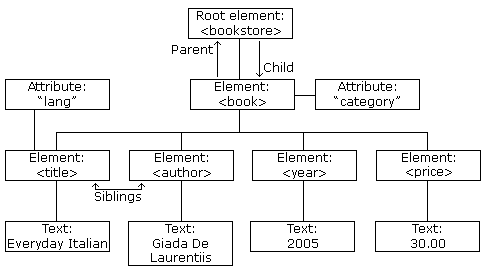
\includegraphics[width=\textwidth]{figures/nodetree}
\caption{Raamatupoe hierarhiline struktuur \citep{XML}}
\end{figure}

Joonise 1 kujutamine XML-kujul \citep{XML}:\\


\begin{lstlisting}
<?xml version="1.0" encoding="UTF-8"?>
<bookstore>
  <book category="cooking">
    <title lang="en">Everyday Italian</title>
    <author>Giada De Laurentiis</author>
    <year>2005</year>
    <price>30.00</price>
  </book>
  <book category="children">
    <title lang="en">Harry Potter</title>
    <author>J K. Rowling</author>
    <year>2005</year>
    <price>29.99</price>
  </book>
  <book category="web">
    <title lang="en">Learning XML</title>
    <author>Erik T. Ray</author>
    <year>2003</year>
    <price>39.95</price>
  </book>
</bookstore>
\end{lstlisting}

XML-i võib vaadata kui reeglite kogumikku, milles talletatakse informatsiooni semantiliste märgendite abil. Märgendid (\emph{tags}) on \emph{<>} märkide vahel olevad muutujad ja igal märgendil peab olema lõpumärgend (nt \emph{<bookstore>} ja \emph{</bookstore>}). XML dokument koosneb kolmest osast: proloog, dokumendi element ja epiloog. Faili alustatakse proloogiga, mis defineerib XML-i versiooni ja kasutatava kodeeringu. Dokumendi element on juurelement, mida saab olla vaid üks. Joonise 1 juurelement on \emph{<bookstore>}, mille alluvaks on elemendid \emph{<book>}. Märgenditel võib olla atribuut kui ka sisu, kuid need pole ilmtingimata kohustuslikud. Selles XML-koodijupis on raamatutel defineeritud ka atribuut \emph{category}, mille väärtus oleneb raamatu valdkonnast. Elemendi \emph{<book>} alluvateks on \emph{<title>}, \emph{<author>}, \emph{<year>} ja \emph{<price>}, mis on omakorda teineteise kolleegid. Kõigil neil elementidel on sisu ja elemendil \emph{<title>} on ka atribuut \emph{lang}, mille väärtuseks on keel. Viimane rida (\emph{</bookstore>}) ütleb, et see on juurelemendi lõpp ja ühtlasi ka dokumendi keha lõpp. See tähendab, et rohkem raamatuid selles raamatupoes ei eksisteeri. \citep{XML}

Märgendite abil pannakse paika andmete loogiline struktuur. XML-il pole eeldefineeritud märgendeid. Seega igal inimesel on võimalik defineerida oma vajadustele vastav struktuur ehk süntaks, mis paneb paika elemendi nimetused ja järjestuse. Oluline on, et kasutaja poolt defineeritud süntaks vastaks XML-i rangetele reeglitele:

\begin{enumerate}
    \item eksisteerib juurelement;
    \item elementidel peab olema lõpumärgend;
    \item elementide pesitsemine (\emph{nesting}) on rangelt määratletud;
    \item atribuutide väärtused peavad olema jutumärkides.
    \citep{XML}
\end{enumerate}

Kui kasutaja loob enda märgenduse, siis XML-protsessoril pole võimalik selle valiidsuses veenduda, sest pole midagi millegagi võrrelda. Selleks tuleb kasutajal XML-dokumendis defineerida kasutatav süntaks. XML-dokumentide valideerimiseks on kaks viisi: dokumenditüübi definitsioon (\emph{document type definition} -- DTD) ja XML skeema (\emph{XML schema}). Nende asukoht on vahetult peale XML-versiooni deklaratsiooni ja kindlasti enne dokumendi keha. Juhul kui XML-dokument on DTD või XML skeemaga vastavuses, siis on ka XML-dokument kehtiv. \citep{XML}

\subsection{Tööprotsess}

Magistritöö eesmärk on luua eesti morfoloogiliselt märgendatud lapsekeele korpus, kuhu on koondatud kõik CHILDES-i eesti keele alamkorpused. Esialgne plaan oli konverteerida omalkäel kõik CHAT-failid XML-kujule, kuid sellega tekkisid mõningad tagasilöögid. Selleks, et CHAT-faile XML-kujule konverteerida, oleks tarvis, et kõik alamkorpused oleksid ühtsel kujul transkribeeritud ja kodeeritud. Peatükis 5.4 tõin välja mõned näited sellest, kui ebajärjepidevalt on seda tehtud. Isegi, kui korpused oleksid olnud standartsel kujul, siis oleks konverteerimisskripti tegemine muutunud väga keeruliseks ja ülejõukäivaks ülesandeks. Põhjus seisneb selles, et CHAT-käsiraamatus on väga suur ja lai valik kodeeringuid, mida on paraku ühel inimesel raske hallata, vt näide (5).

(5)
\begin{description}
    \item*CHI:   see kifiir \textbf{[:} kefiir\textbf{]} .
    \item*MOT:   kus sa $\pmb{+/}$.
    \item*CHI:   $\pmb{+<}$ \textbf{(}h\textbf{)}akkas põlema .
    \item*MOT:   see ei ole kefiir ju .
    \item*CHI:   kefiir . $\pmb{[+}$ sr\textbf{]}
    \item*MOT:   see on piim .
    \item*FAT:   mis see kook teeb ?
    \item*FAT:   tuleb ära panna $\pmb{[=}$ visata\textbf{]} või ?
    \item*MOT:   mina ei tea , vist jah .
    \item*CHI:   kuidas emme küpsetab saia , lihat\textbf{@n} \textbf{[*]} .
    \item\%err:   lihat=liha \$MOR
    \item*FAT:   saia ei ei küpseta .
    \item*FAT:   kartulit küpsetame , \textbf{(.)} ahjus .
    \item*CHI:   $\pmb{+<}$ saia .
    \item*CHI:   lihat\textbf{@n} \textbf{[*]} . $\pmb{[+}$ \textbf{sr]}
    \item\%err:   lihat=liha \$MOR
    \item*FAT:   liha ka jah .
    \item*CHI:   lihat\textbf{@n} \textbf{[*]} . $\pmb{[+}$ \textbf{sr]}
    \item\%err:   lihat=liha \$MOR
    \item\%act:   MOT koorib sibulat
    \item...
    \item*CHI:   Atu \textbf{[:} Andreas\textbf{]} sõi $\pmb{+...}$
    \item*CHI:   $\pmb{+}$\textbf{"} a .
    \item...
    \item*CHI:   käpad \textbf{(}h\textbf{)}aige \textbf{[*]} \textbf{[$\pmb{/]}$} käpad \textbf{(}h\textbf{)}aige \textbf{[*]} .
    \item (Vija; 20018.cha)
\end{description}


Näites (5) on näha, kui mitmekesine võib ühes transkriptsioonis kodeeringute kasutus olla. On arusaadav, et iga uurija transkribeerib ja kodeerib lindistusi lähtuvalt enda eesmärkidest. Ühest käest on hea, et CHAT-käsiraamatus on niivõrd detailne kodeering, kuid teisalt võib selles orienteerumine vägagi raskeks osutuda. Kuna sellise konverteerimisskripti kirjutamise töömaht oleks selle magistritöö kirjutamise jaoks liiga töömahukaks osutunud, siis tuli leida uus lahendus. 

\begin{figure}[H]
    \centering
    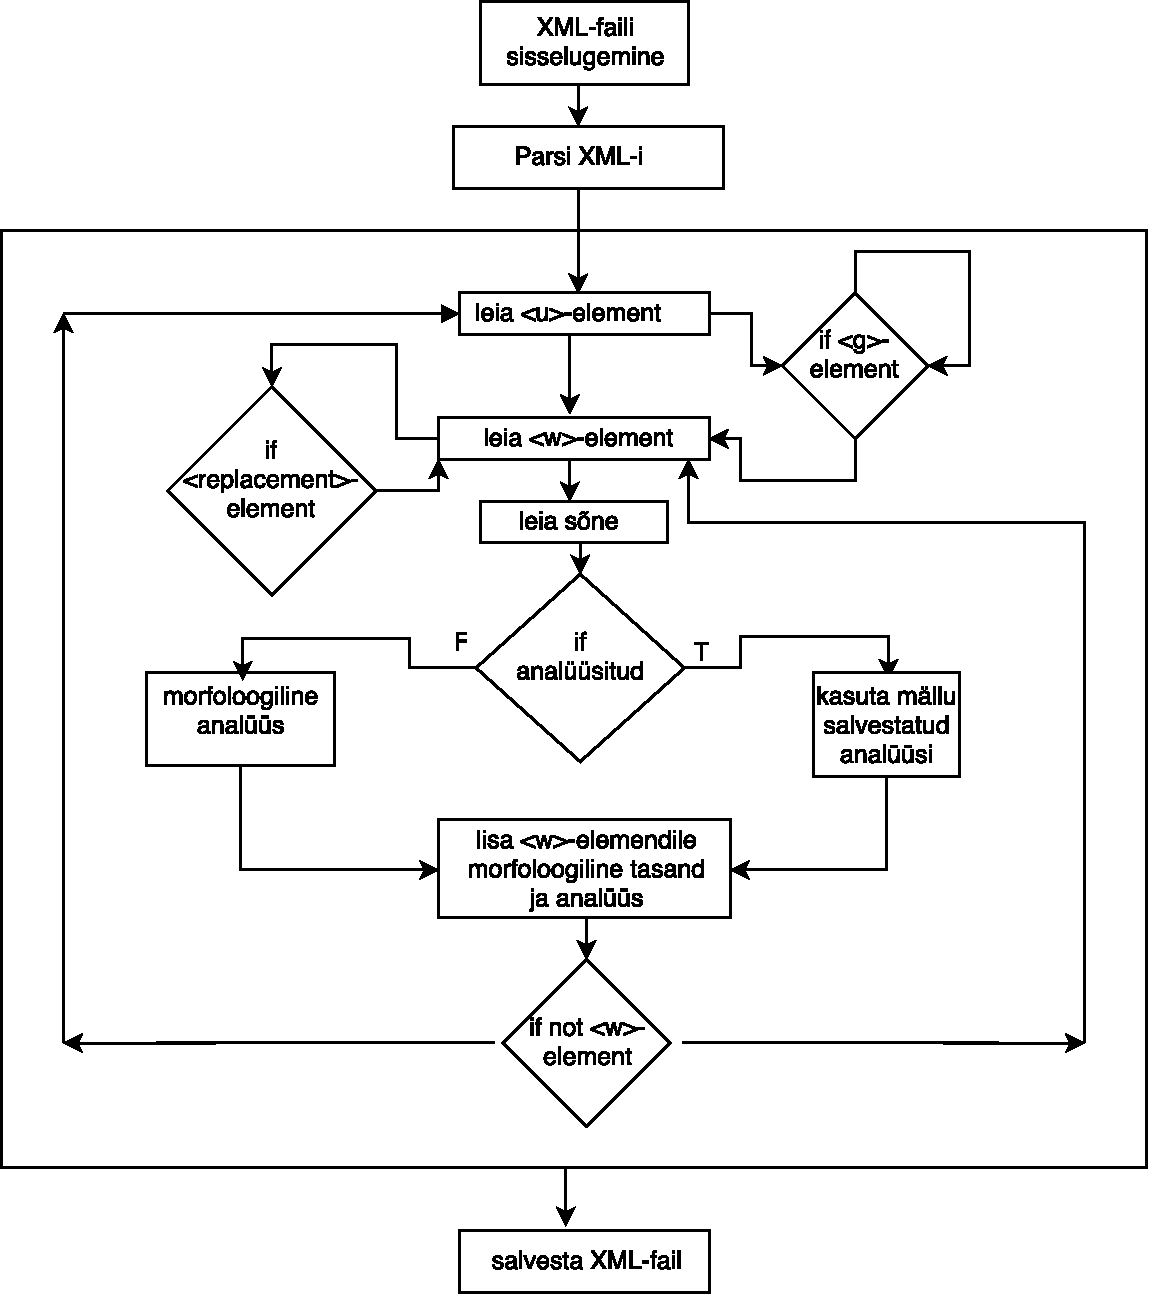
\includegraphics[width=\textwidth]{toovoog}
    \caption{Töövoog}
\end{figure}


\section{Kokkuvõte}

Seminaritöös kirjeldati korpuse olemust ja selle tähtsust keeleuurijale. Korpuse mõte on seisneb selles, et sealt võimalikult lihtsalt olulist infot kätte saada, aga kahjuks korpuste standardiseerimine ja loomine pole nii lihtne töö. Kõik algab algmaterjalist. 

Selle töö eesmärk oli lühidalt tutvustada ja näidata, et selleks, et lapsekeele korpust luua, tuleks transkriptsioonides esmalt selgeks teha, et mida ja kuidas märgendada. Kui see on selgeks tehtud, siis tuleks dialoogide transkribeerimisel sellest ka kinni pidada ja teha seda järjepidevalt. Eelmises peatükis kirjeldasin vaid mõningaid transkriptsioonidega seotud probleeme. Paraku on nii, et see esimene tase (transkriptsioon) mõjutab oluliselt vahepealseid tasandeid (standardiseerimine ja morfoloogilise info lisamine), mis omakorda mõjutavad lõpliku morfoloogiliselt märgendatud korpuse kvaliteeti.

\newpage
\cleardoublepage
\phantomsection
\addcontentsline{toc}{section}{\refname}
\bibliographystyle{dcu}
\bibliography{viited}

\end{document}


